%-----------------------------------------------------------------------------%
\chapter{ANALISIS DAN PERANCANGAN SISTEM}
%-----------------------------------------------------------------------------%

%
\vspace{4.5pt}

\noindent Bab ini memaparkan analisis masalah yang diatasi berserta pendekatan dan alur kerja dari perangkat lunak yang dikembangkan, mengimplementasikan metode yang digunakan dan hasil yang akan ditampilkan.
\\
\section{Analisis Masalah}
\noindent Pada bab 1 telah dijelaskan bahwa penelitian mengenai sistem pengenalan plat nomor kendaraan merupakan bidang yang masih berkembang dan implementasinya memegang peranan penting dalam bidang transportasi. Pada penelitian ini, metode yang akan digunakan adalah \textit{Canny Detector} dan \textit{Hough Transform} untuk mendeteksi lokasi plat kendaraan, kemudian menggunakan metode \textit{Histogram of Oriented Gradient} untuk mengekstraksi fitur dari citra karakter dari plat nomor yang sudah disegmentasi dengan menghitung grafik horizontal pita, kemudian dilakukan klasifikasi dengan menggunakan metode \textit{Support Vector Machine}.
%\noindent Pada bab 1 telah dijelaskan bahwa mendeteksi manusia merupakan bidang yang masih berkembang dan implementasinya sangat dibutuhkan di berbagai bidang. Pada penelitian ini, penulis menggunakan citra RGB-D agar tetap memiliki hasil yang baik pada kondisi pencahayaan yang relatif gelap. Dengan menggunakan citra kedalaman akan sangat membantu dalam proses deteksi manusia dalam tahap awal, \textit{training}, ataupun tahap \textit{testing}. Penerapan \textit{Convolutional Neural Network} untuk mendeteksi manusia dan Kalman \textit{filter} untuk melacak manusia yang telah terdeteksi. Bagian tubuh manusia yang akan dideteksi adalah bagian tubuh atas sehingga tetap dapat mendeteksi manusia bila terdapat citra manusia yang tertutup atau hanya tampak sebagian.

\noindent Masukan untuk sistem deteksi dan pengenalan plat nomor kendaraan ini adalah citra yang ditangkap oleh kamera DSLR Canon EOS 500 D dan Canon EOS 550 D beresolusi 15 dan 18 megapiksel. Citra tangkapan kemudian akan diubah resolusinya menjadi 1024 $\times$ 640 piksel. Setiap citra masukan berisi bagian depan dari kendaraan yang memiliki plat nomor kendaraan.

\noindent Keluaran atau hasil dari sistem akan berupa teks hasil dari pengenalan karakter pada citra plat nomor kendaraan masukkan.\\ 

\section{Kerangka Pemikiran}
\noindent Berikut ini adalah kerangka pemikiran dari metode yang diusulkan untuk melakukan deteksi plat nomor kendaraan dan melakukan pengenalan karakter pada citra karakter yang terdapat pada plat nomor.\\

\begin{adjustbox}{width=1\textwidth}
	\noindent\begin{minipage}{\linewidth}
	\framebox[\textwidth]{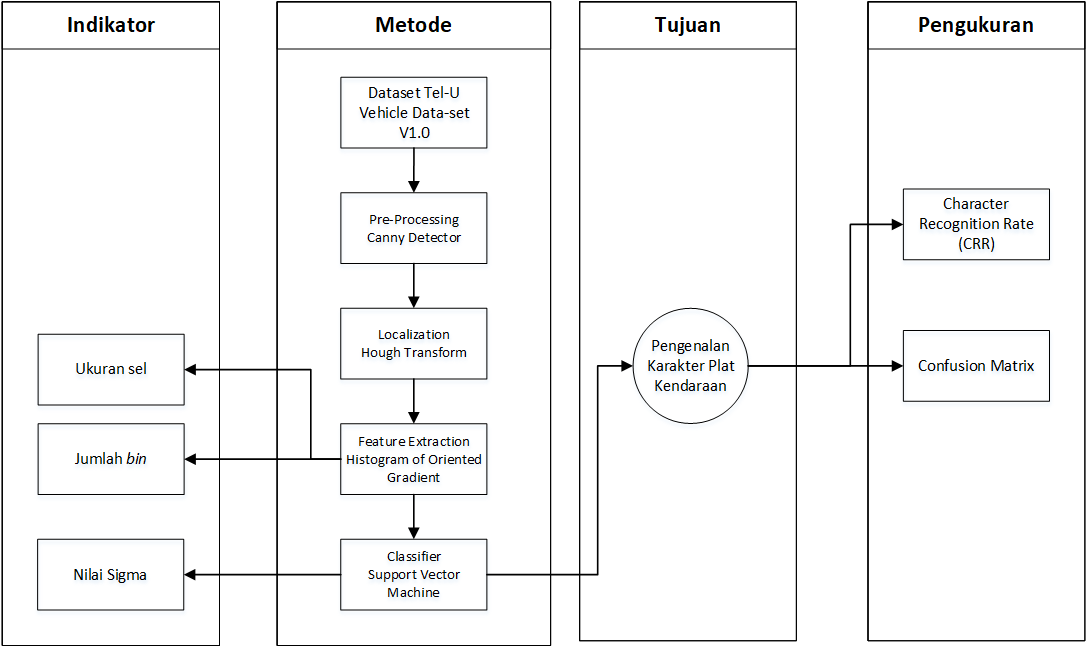
\includegraphics[width=13cm]{images/KerangkaPemikiran.png}}
	\captionof{figure}{Kerangka Pemikiran}
	\label{fig:KerangkaPemikiran}
\end{minipage}
\end{adjustbox}

\noindent Seperti pada gambar \ref{fig:KerangkaPemikiran}, terdapat beberapa variabel indikator yang memengaruhi hasil dan perlu dilakukan penyesuaian, seperti ukuran sel pada metode \textit{Histogram of Oriented Gradient}, jumlah \textit{bin} yang menentukan batasan sudut yang digunakan, dan jumlah data \textit{training} untuk \textit{classifier} \textit{Support Vector Machine}. Penelitian ini memiliki dua tujuan, yaitu untuk melihat hasil akurasi deteksi plat nomor dan akurasi pengenalan karakter pada plat nomor dengan menggunakan \textit{confusion matrix}.\\

\section{Urutan Proses Global}
\noindent Dalam sistem pengenalan plat nomor kendaraan terbagi atas dua proses yaitu proses \textit{training} dan proses \textit{testing}. Proses \textit{training} dilakukan untuk mendapatkan kelas-kelas dari karakter-karakter yang akan dikenali. Proses \textit{testing} dilakukan untuk menghitung hasil yang berupa akurasi dari pengenalan karakter pada plat nomor kendaraan.\\

\subsection{Proses \textit{Training}}

\begin{adjustbox}{width=1\textwidth}
	\noindent\begin{minipage}{\linewidth}
		\framebox[\textwidth]{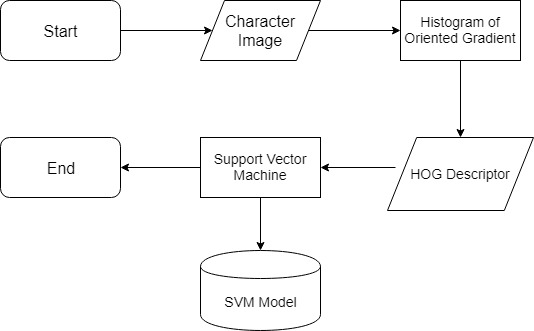
\includegraphics[width=12cm]{images/FlowchartTraining.jpg}}
		\captionof{figure}{\textit{Flowchart Training} Sistem Pengenalan Plat Nomor Kendaraan\\}
		\label{fig:FlowchartTraining}
	\end{minipage}
\end{adjustbox}

Berikut ini adalah uraian dari \textit{flowchart} pada gambar \ref{fig:FlowchartTraining} yang dilakukan dalam penelitian ini:
\begin{enumerate}
\item Citra yang menjadi masukan yaitu dari \textit{dataset English Font} yang berasal dari \textit{The Chars 74K image dataset} yang berisi kumpulan jenis karakter dari komputer dengan 4 variasi, yaitu citra karakter miring (\textit{Italic}), citra karakter tebal (\textbf{Bold}), dan citra karakter normal. Citra karakter memiliki ukuran 128 $\times$ 128 piksel. Citra karakter berwarna hitam dengan latar belakang berwarna putih. Kumpulan karakter yang digunakan adalah karakter angka dari 0 sampai dengan 9 dan karakter huruf kapital dari A sampai dengan Z, karakter huruf kecil tidak digunakan karena pada plat nomor kendaraan tidak menggunakan karakter huruf kecil.
\item \textit{Histogram of Oriented Gradient} berfungsi untuk mendapatkan fitur dari dari citra masukan. Hasil dari ekstraksi fitur dengan menggunakan HOG adalah \textit{HOG descriptor}, yang mendeskripsikan distribusi dari gradien berarah pada suatu area citra.
\item Ukuran sel dan blok yang digunakan untuk proses ekstraksi fitur dengan menggunakan \textit{HOG} adalah 8 $\times$ 8 piksel untuk ukuran sel dan 4 $\times$ 4 sel dan jumlah \textit{bin} yang digunakan pada tahap pembuatan \textit{histogram} adalah 9 dimulai dari 0 derajat hingga 180 derajat.
\item \textit{Support Vector Machine} (SVM) digunakan untuk mengklasifikasikan fitur-fitur yang sudah didapatkan ke dalam kelas-kelas dari karakter yang akan dikenali. Hasil dari klasifikasi ini nantinya akan disimpan ke dalam bentuk berkas.\\
\end{enumerate}

%\begin{spacing}{1}
%\noindent\rule{\textwidth}{1.5pt}
%\textbf{Algoritme \textit{Convolutional Neural Network} tahap %\textit{Training}}
%\begin{enumerate}
%\item Masukkan citra kedalaman yang telah melewati tahap %\textit{pre-processing}.
%\item Inisialisasi nilai setiap \textit{neuron}/\textit{filter}, \textit{learning rate}, dan \textit{epoch}.
%\item Lakukan proses konvolusi (perkalian citra masukan dengan \textit{neuron}), didapatkan \textit{induced local field} dengan persamaan \ref{eq:InducedLocalField}.
%\item Gunakan fungsi aktivasi \textit{rectified linear units} (ReLUs) menggunakan persamaan \ref{eq:RELU}.
%\item Lakukan proses \textit{subsampling} dengan \textit{max pooling} dari nilai pada lapisan sebelumnya. Catat juga indeks yang menyimpan nilai maksimal.
%\item Lakukan proses konvolusi (perkalian masukan dengan \textit{neuron}), didapatkan \textit{induced local field} dengan persamaan \ref{eq:InducedLocalField}.
%\item Gunakan fungsi aktivasi \textit{rectified linear units} (ReLUs) menggunakan persamaan \ref{eq:RELU}.
%\item Lakukan proses \textit{subsampling} dengan \textit{max pooling} dari nilai pada lapisan sebelumnya. Catat juga indeks yang menyimpan nilai maksimal.
%\item Pada lapisan \textit{fully connected}, ubah masukan menjadi vektor (matriks 1 dimensi).
%\item Kalkulasi vektor dengan \textit{filter} dari setiap jenis objek.
%\item Kalkulasi dengan \textit{softmax} menggunakan persamaan \ref{eq:Softmax}, sehingga didapatkan besar probabilitas jenis objek.
%\item Kalkulasi nilai \textit{error} dengan \textit{loss function} \textit{cross-entropy} menggunakan persamaan \ref{eq:crossEntropy}.
%\item Kalkulasi nilai gradien pada setiap lapisan secara terbalik atau mundur.
%\item Kalkulasi ulang nilai pada \textit{neuron} yaitu \textit{weight}/\textit{parameter} sesuai dengan nilai gradiennya masing-masing.
%\item Ulangi langkah 3-14 hingga mencapai \textit{epoch} yang ditentukan.
%\item Simpan model CNN yang berisi \textit{descriptor} CNN beserta nilai \textit{neuron} untuk digunakan pada tahap \textit{testing}.
%\end{enumerate}
%\noindent\rule{\textwidth}{1pt}
%\end{spacing}

%\noindent Dengan \textit{hyperparameter} yang digunakan pada algoritme \textit{Convolutional Neural Network} adalah sebagai berikut:
%\begin{enumerate}
%\item Ukuran \textit{padding} pada seluruh lapisan adalah 0.
%\item Inisialisasi seluruh nilai \textit{kernel} pada lapisan \textit{convolution} dan \textit{fully connected} adalah nilai acak dengan rentang nilai antara -0.005 hingga 0.005.
%\item Inisialisasi seluruh nilai \textit{bias} pada lapisan \textit{convolution} dan \textit{fully connected} bernilai 0.
%\item Pada lapisan \textit{convolution}, ukuran \textit{filter} adalah 5 $\times$ 5 dan \textit{stride} adalah 1.
%\item Pada lapisan \textit{subsampling}, ukuran \textit{kernel} 2 $\times$ 2 dan \textit{stride} adalah 2.
%\item Pada lapisan \textit{fully connected}, ukuran \textit{filter} adalah 1 $\times$ 117, yaitu hasil dari vektorisasi menjadi 1 dimensi dari ukuran 9 $\times$ 13.
%\end{enumerate}

%\begin{spacing}{1}
%\noindent\rule{\textwidth}{1.5pt}
%\textbf{Algoritme \textit{Backpropagation Convolutional Neural Network}}
%\begin{enumerate}
%\item Kalkulasi nilai gradien lokal dari hasil \textit{softmax} dengan persamaan \ref{eq:localGradientOutputSoftmax}.
%\item Kalkulasi nilai gradien lokal, gradien kernel, dan gradien bias pada lapisan \textit{fully connected} dengan persamaan \ref{eq:localGradientOutput} dan hasil dari nilai gradien \textit{softmax} sebelumnya.
%\item Kalkulasi nilai gradien lokal pada lapisan \textit{subsampling} dengan persamaan \ref{eq:localGradientPooling}. Nilai yang teruskan adalah nilai gradien lokal yang merupakan indeks maksimal yang telah dicatat sebelumnya saat proses \textit{forward propagation}.
%\item Kalkulasi nilai gradien lokal, gradien kernel, dan gradien bias pada lapisan \textit{convolution} dengan persamaan \ref{eq:localGradientHidden} dan persamaan \ref{eq:derivativeReLU} sebagai turunan fungsi aktivasi ReLU.
%\item Kalkulasi nilai gradien lokal pada lapisan \textit{subsampling} dengan persamaan \ref{eq:localGradientPooling}. Nilai yang teruskan adalah nilai gradien lokal yang merupakan indeks maksimal yang telah dicatat sebelumnya saat proses \textit{forward propagation}.
%\item Kalkulasi nilai gradien lokal, gradien kernel, dan gradien bias pada lapisan \textit{convolution} dengan persamaan \ref{eq:localGradientHidden} dan persamaan \ref{eq:derivativeReLU} sebagai turunan fungsi aktivasi ReLU.
%\item Perbarui nilai \textit{weight} and bias dengan persamaan \ref{eq:weightCorrection} sesuai dengan nilai gradien lokal yang telah dikalkulasi pada setiap lapisan (seluruh lapisan jenis \textit{convolution} dan \textit{fully connected}).
%\end{enumerate}
%\noindent\rule{\textwidth}{1pt}
%\end{spacing}

\subsection{Proses \textit{Testing}}

\begin{adjustbox}{width=1\textwidth}
	\noindent\begin{minipage}{\linewidth}
		\framebox[\textwidth]{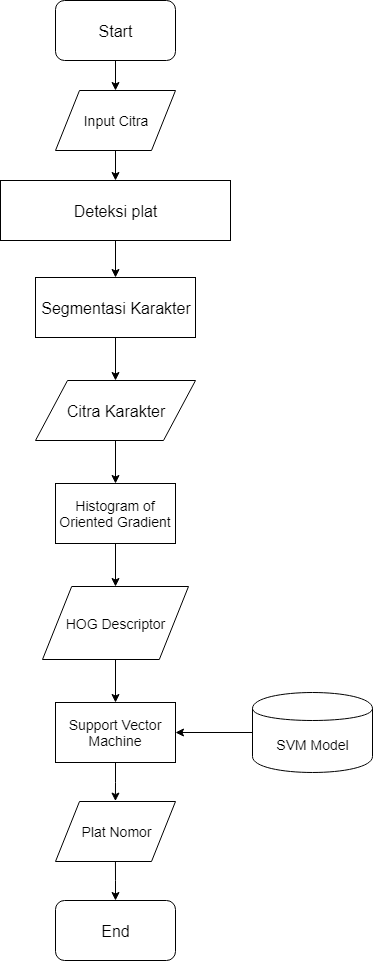
\includegraphics[width=7cm]{images/FlowchartTesting.png}}
		\captionof{figure}{\textit{Flowchart Testing} Sistem Deteksi dan Pengenalan Plat Nomor\\}
		\label{fig:FlowchartTesting}
	\end{minipage}
\end{adjustbox}

\noindent Pada gambar \ref{fig:FlowchartTesting} terlihat urutan proses \textit{testing}. Pada proses \textit{testing} terdapat beberapa proses yang sama seperti pada proses \textit{training}. Berikut ini adalah uraian dari \textit{flowchart} pada gambar \ref{fig:FlowchartTesting} yang dilakukan dalam penelitian ini:
\begin{enumerate}
\item Citra pengujian yang digunakan didapatkan dari \textit{dataset} plat nomor kendaraan Universitas Telkom yang bernama \textit{Tel-U Vehicle Data-set V1.0}, penggunaan dari dataset ini sesuai dengan perizinan dari institusi yang bersangkutan.
\item Citra yang akan menjadi input dari \textit{HOG} adalah citra hasil dari segmentasi karakter pada citra plat kendaraan pada tahapan deteksi lokasi plat nomor kendaraan.
\item Ukuran dari sel dan blok yang digunakan untuk proses ekstraksi fitur dengan menggunakan \textit{HOG} adalah sama dengan yang digunakan ketika pada tahap \textit{training}.
\item Pada tahap \textit{testing} model SVM yang digunakan diambil dari berkas yang merupakan hasil keluaran dari SVM pada tahap \textit{training}.
\item Hasil keluaran akan berupa sebuah \textit{string} yang menunjukkan kumpulan karakter yang berhasil dikenali oleh sistem.\\
\end{enumerate}

%\begin{spacing}{1}
%\noindent\rule{\textwidth}{1.5pt}
%\textbf{Algoritme \textit{Convolutional Neural Network} tahap \textit{Testing}}
%\begin{enumerate}
%\item Masukkan citra kedalaman yang merupakan kandidat manusia yang telah melewati tahap \textit{pre-processing}.
%\item Muat dan gunakan model CNN dari tahap \textit{training}.
%\item Kalkulasi citra masukan menggunakan model belajar CNN sebelumnya.
%\item Hitung hasil probabilitas dari citra masukan.
%\end{enumerate}
%\noindent\rule{\textwidth}{1pt}\\
%\end{spacing}

%\begin{spacing}{1}
%\noindent\rule{\textwidth}{1.5pt}
%\textbf{Algoritme Kalman \textit{Filter} tahap \textit{Testing}}\\
%\noindent Untuk setiap nilai $x_{1}$, $y_{1}$, $x_{2}$, dan $y_{2}$, lakukan prosedur berikut secara terpisah:
%\begin{enumerate}
%\item Inisialisasi nilai \textit{bounding box} awal, \textit{covariance error} ($P_{k}$), \textit{noise} ($R_{k}$) awal.
%\item Lakukan pembaruan informasi pada iterasi awal untuk adaptasi agar \textit{error} lebih rendah, yaitu kalkulasi Kalman \textit{gain}, estimasi baru, \textit{covariance error} baru.
%\item Setelah dilakukan adaptasi, kalkulasi prediksi nilai posisi dan \textit{covariance error}. Hasil prediksi nilai posisi dapat digunakan untuk membentuk \textit{bounding box}.
%\item Perbarui informasi dengan melakukan pembaruan informasi, yaitu kalkulasi Kalman \textit{gain}, estimasi baru, \textit{covariance error} baru.
%\item Ulangi langkah 3-4 hingga mencapai jumlah pengulangan tertentu.
%\item Ulang dari langkah pertama untuk memperbarui kondisi baru.
%\end{enumerate}
%\noindent\rule{\textwidth}{1pt}\\
%\end{spacing}

\section{Analisis Manual}
\noindent Pada bagian ini dilakukan analisis tahapan proses dengan melakukan perhitungan manual.\\

\subsection{\textit{Dataset}}
\noindent Dari \textit{The Chars 74K image dataset} untuk tahap \textit{training} akan digunakan citra karakter angka dari 0 sampai dengan 9 dan karakter huruf kapital A sampai dengan Z. Terlihat contoh citra karakter yang ditunjukan pada gambar \ref{fig:ContohCitraDatasetPakai} merupakan contoh karakter angka dan huruf kapital yang akan dipakai. Sedangkan pada gambar \ref{fig:ContohCitraDatasetTakPakai}, gambar tersebut menunjukkan contoh citra karakter yang tidak akan dipakai, yaitu citra karakter tipis, miring, dan karakter huruf kecil. Tidak digunakannya karakter-karakter tersebut dikarenakan pada plat nomor Indonesia, karakter yang digunakan hanyalah karakter huruf kapital dan angka dalam bentuk tegak dan tebal.

\begin{adjustbox}{width=1\textwidth}
	\noindent\begin{minipage}{\linewidth}
		\framebox[\textwidth]{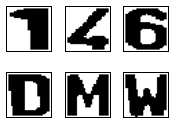
\includegraphics[width=8cm]{images/CitraDatasetPakai.PNG}}
		\captionof{figure}{Contoh citra karakter yang digunakan untuk tahap \textit{training}\\}
		\label{fig:ContohCitraDatasetPakai}
	\end{minipage}
\end{adjustbox}

\begin{adjustbox}{width=1\textwidth}
	\noindent\begin{minipage}{\linewidth}
		\framebox[\textwidth]{
\includegraphics[width=12cm]{images/CitraDatasetTakPakai.PNG}}
		\captionof{figure}{Contoh citra karakter yang tidak digunakan\\}
		\label{fig:ContohCitraDatasetTakPakai}
	\end{minipage}
\end{adjustbox}\\


\subsection{Tahap Pendeteksian Lokasi Plat Nomor}
\noindent Skema alur dari tahap pendeteksian lokasi plat nomor adalah:

\begin{adjustbox}{width=1\textwidth}
	\noindent\begin{minipage}{\linewidth}
		\framebox[\textwidth]{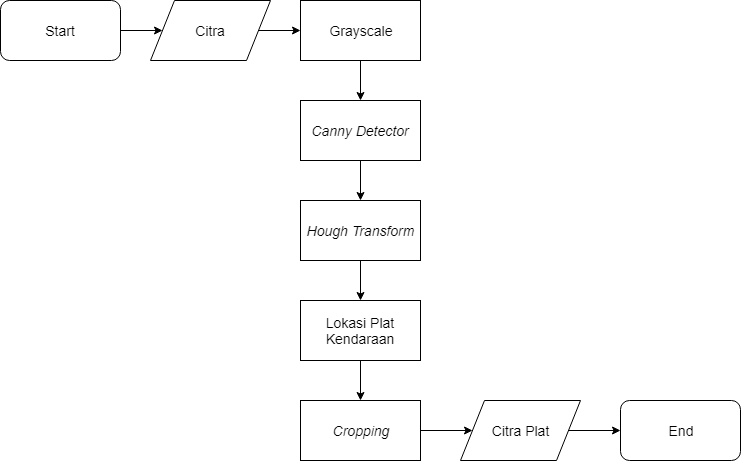
\includegraphics[width=13cm]{images/FlowchartDeteksiPlat.png}}
		\captionof{figure}{Skema Alur Pendeteksian Plat\\}
		\label{fig:SkemaAlurPendeteksianPlat}
	\end{minipage}
\end{adjustbox}\\

\subsubsection{\textit{Grayscale}}
\noindent Proses pertama adalah mengubah citra masukan menjadi citra \textit{grayscale}, tujuan dari \textit{grayscaling} citra adalah untuk menghilangkan informasi warna dari setiap piksel citra. Untuk menghitung nilai derajat keabuan setiap piksel, diperoleh dengan menggunakan persamaan \ref{eq:grayscale}.

\noindent Di bawah merupakan contoh matriks citra asli dengan 3 \textit{channel} warna yaitu \textit{Red}, \textit{Green}, dan \textit{Blue} berukuran 5 $\times$ 5 piksel yang diambil dengan menggunakan \textit{image tools} dari aplikasi \textit{MatLab} \\

\begin{adjustbox}{width=1\textwidth}
	\noindent\begin{minipage}{\linewidth}
		\framebox[\textwidth]{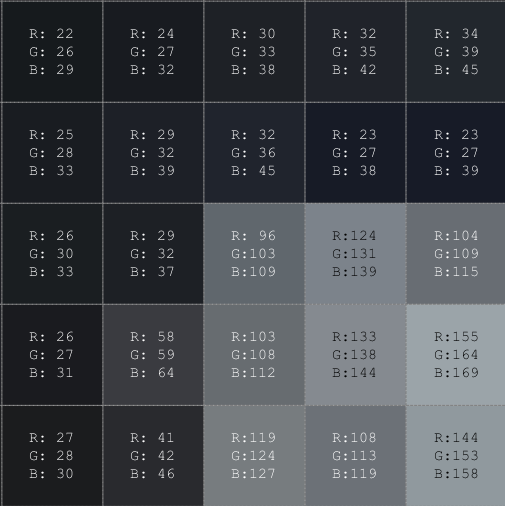
\includegraphics[width=8cm]{images/CitraMatriksAsal.PNG}}
		\captionof{figure}{Matriks Citra Asal berukuran 5 $\times$ 5\\}
		\label{fig:MatriksCitraAsal}
	\end{minipage}
\end{adjustbox} \\

\noindent Dengan menggunakan persamaan \ref{eq:grayscale}, maka nilai matriks citra \textit{grayscale} pada titik (3,3) akan menjadi sebagai berikut:
\begin{table}[H]
	\begin{adjustbox}{width=1\textwidth}
		\begin{tabular}{|p{13.55cm}|}
			\hline
			\begin{equation}\nonumber
			\begin{aligned}
			Matriks[3,3] &= (0.299 * 133) + (0.587 * 138) + (0.114 * 144) \\
						 &= 137.189 \approx 137 
			\end{aligned}
			\end{equation}\\
			\hline
		\end{tabular}
	\end{adjustbox}
\end{table}

\noindent Perhitungan di atas dilakukan terhadap seluruh nilai matriks citra asal dan hasilnya adalah matriks citra berukuran 5 $\times$ 5 dengan satu nilai derajat keabuan.

\begin{adjustbox}{width=1\textwidth}
	\noindent\begin{minipage}{\linewidth}
		\framebox[\textwidth]{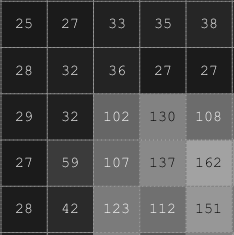
\includegraphics[width=6cm]{images/CitraMatriksGrayscale.PNG}}
		\captionof{figure}{Matriks Citra Hasil \textit{Grayscale}\\}
		\label{fig:MatriksCitraGrayscale}
	\end{minipage}
\end{adjustbox} \\

\subsubsection{Deteksi Tepi Canny}
\noindent Proses deteksi tepi dapat dilakukan terhadap sebuah citra biner. Pada penelitian ini, metode \textit{Canny Edge Detection} digunakan untuk mendapatkan tepian. Berikut adalah algoritme dari metode \textit{Canny Edge Detection} untuk mendapatkan tepian.

\begin{enumerate}[leftmargin=16pt]
\item Citra masukkan diperhalus dengan menggunakan \textit{Gaussian Filter} untuk membuang derau.
\item Lakukan operasi perhitungan gradien menggunakan operator Sobel, Prewitt, atau Robert untuk mendapatkan tepian yang tebal.
\item Untuk menipiskan tepian yang didapat dari operasi sebelumnya maka teknik \textit{Non-Maxima Suppression} dilakukan dengan mencari nilai maksimum pada tepian.
\item Buat 2 nilai \textit{threshold} yaitu \textit{high threshold} dan \textit{low threshold} untuk menentukan piksel mana yang masuk dalam kategori tepian kuat, tepian lemah, dan bukan tepian. Jika nilai dari piksel tersebut di atas \textit{high threshold}, maka piksel tersebut masuk ke dalam kategori tepian kuat, apabila nilai piksel berada di antara batas \textit{high threshold} dan \textit{low threshold}, maka piksel tersebut masuk ke dalam kategori tepian lemah, selebihnya akan masuk ke dalam kategori bukan tepian.
\item Tahapan terakhir adalah \textit{Edge Linking} untuk menghubungkan tepian lemah dengan tepian kuat. Apabila piksel tepian lemah memiliki tetangga piksel (terhubung), maka piksel tersebut akan menjadi tepian.
\end{enumerate}
%\noindent Pada bagian ini menjelaskan urutan langkah kerja pada proses Deteksi Tepi Canny. Gambar \ref{fig:FlowchartCannyDetector} adalah \textit{flowchart} Deteksi Tepi Canny.
%
%\begin{adjustbox}{width=1\textwidth}
%	\noindent\begin{minipage}{\linewidth}
%		\framebox[\textwidth]{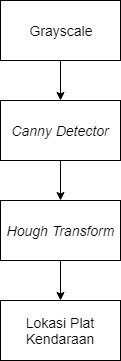
\includegraphics[width=3cm]{images/FlowchartDeteksiPlat.jpg}}
%		\captionof{figure}{\textit{Flowchart} Deteksi Tepi Canny\\}
%		\label{fig:FlowchartCannyDetector}
%	\end{minipage}
%\end{adjustbox}\\

\noindent Berdasarkan algoritme yang sudah dijabarkan, hal pertama yang dilakukan untuk deteksi tepi Canny adalah dengan melakukan \textit{smoothing} pada citra dengan menggunakan turunan pertama pertama dari \textit{Gauss} dengan besar \textit{kernel} 3 $\times$ 3 dan nilai dari $\sigma$ = 1 untuk menghilangkan \textit{noise}.
\begin{gather*}
\textit{Matriks Gauss Kernel}
=
\begin{bmatrix}
0.077847 & 0.123317 & 0.077847 \\
0.123317 & 0.195346	& 0.123317 \\
0.077847 & 0.123317 & 0.077847
\end{bmatrix}
\label{eq:MatriksGaussKernel}
\end{gather*} 

\noindent\textit{Kernel} seperti pada persamaan Matriks \textit{Gauss Kernel} di atas dikonvolusikan ke dalam citra untuk mendapatkan sebuah nilai baru. Sebagai contoh apabila diambil area pada sebuah citra sebesar 5 $\times$ 5 piksel seperti pada gambar \ref{fig:MatriksCitra} yang kemudian dikonvolusikan menggunakan \textit{Gauss Kernel}.

\begin{table}[H]
	\centering
	\begin{small}
		\begin{tabular}{|p{1cm}|p{1cm}|p{1cm}|p{1cm}|p{1cm}|}
			\hline
			25 & 27 & 33 & 35 & 38 \\
			\hline
			28 & 32 & 36 & 27 & 27 \\
			\hline
			29 & 32 & 102 & 130 & 108 \\
			\hline
			27 & 59 & 107 & 137 & 162 \\
			\hline
			28 & 42 & 123 & 112 & 151 \\\hline
		\end{tabular}
	\end{small}
	\captionof{figure}{Matriks citra ukuran 5 $\times$ 5\\}
	\label{fig:MatriksCitra}
\end{table}

\noindent Maka pada elemen matriks (3,3) nilainya berubah menjadi:
\begin{table}[H]
	\begin{adjustbox}{width=1\textwidth}
		\begin{tabular}{|p{13.55cm}|}
			\hline
			\begin{equation}\nonumber
			\begin{aligned}
			Matriks[3,3] &= (0.077847 * 102) + (0.123317 * 130) + (0.077847 * 108) \\
						 &+ (0.123317 * 107) + (0.195346 * 137) + (0.123317 * 162) \\
						 &+ (0.077847 * 123) + (0.123317 * 112) + (0.077847 * 151)\\
			\end{aligned}
			\end{equation}\\
			\hline
		\end{tabular}
	\end{adjustbox}
\end{table}

\begin{table}[H]
	\begin{adjustbox}{width=1\textwidth}
		\begin{tabular}{|p{13.55cm}|}
			\hline
			\begin{equation}\nonumber
			\begin{aligned}
			Matriks[3,3] &= 127,45534 \approx 127
			\end{aligned}
			\end{equation}\\
			\hline
		\end{tabular}
	\end{adjustbox}
\end{table}

\noindent Sehingga elemen matriks (3,3) berubah nilainya menjadi 127, perhitungan tersebut berlaku untuk semua elemen matriks sisanya, kecuali pada elemen matriks di tepian citra, sehingga seluruh tepian citra sebesar 1 piksel tidak berubah.

\noindent Berdasarkan perhitungan di atas, didapatkan hasil matriks citra hasil konvolusi sebagai berikut:

\begin{table}[H]
	\centering
	\begin{small}
		\begin{tabular}{|p{1cm}|p{1cm}|p{1cm}|p{1cm}|p{1cm}|}
			\hline
			25 & 27 & 33 & 35 & 38 \\
			\hline
			28 & 36 & 48 & 55 & 27 \\
			\hline
			29 & 49 & 77 & 97 & 108 \\
			\hline
			27 & 59 & 97 & 127 & 162 \\
			\hline
			28 & 42 & 123 & 112 & 151 \\\hline
		\end{tabular}
	\end{small}
	\captionof{figure}{Matriks citra ukuran 5 $\times$ 5 hasil konvolusi\\}
	\label{fig:MatriksCitraHasilKonvolusi}
\end{table}

\noindent Tahap selanjutnya adalah perhitungan gradien dengan menggunakan operator gradien sobel. Sebagai contoh dengan area yang sama seperti yang digunakan pada \textit{Gaussian Filter} pada titik(3,3), perhitungan gradien dilakukan sebagai berikut:

\begin{table}[H]
	\begin{adjustbox}{width=1\textwidth}
		\begin{tabular}{|p{15cm}|}
			\hline
			\begin{equation}\nonumber
			\begin{aligned}
			G_{x} &= (-1 * 77) + (0 * 97) + (1 * 108) \\
			 	  &+ (-2 * 97) + (0 * 127) + (2 * 162) \\ 
			 	  &+ (-1 * 123) + (0 * 112) + (1 * 151)\\
			G_{x} &= 188\\
			\end{aligned}
			\end{equation}\\
			\begin{equation}\nonumber
			\begin{aligned}
			G_{y} &= (-1 * 77) + (-2 * 97) + (-1 * 108) \\
				  &+ (0 * 97) + (0 * 127) + (0 * 162) \\
				  &+ (1 * 123) + (2 * 112) + (1 * 151) \\
			G_{y} &= 118\\
			\end{aligned}
			\end{equation}\\
			\begin{equation}\nonumber
			\begin{aligned}
			m &= \sqrt{G_{x}^2 + G_{y}^2} = \sqrt{188^2 + 118^2} = 221.716 \\
			\end{aligned}
			\end{equation}\\
			\begin{equation}\nonumber
			\begin{aligned}
			\theta &= arctan(\frac{118}{188}) = 32.122 \\
			\end{aligned}
			\end{equation}\\
			\hline
		\end{tabular}
	\end{adjustbox}
	\captionof{figure}{Perhitungan gradien dan arah\\}
	\label{fig:PerhitunganGradiendanArah}
\end{table}

\noindent Dari hasil perhitungan di atas, didapatkan informasi bahwa titik (3,3) merupakan tepian yang memiliki arah $32.122^\circ$ dengan \textit{magnitude} sebesar 221.716. Jika \textit{gradient magnitude} lebih dari 255 maka piksel akan menjadi 255 dan jika \textit{gradient magnitude} kurang dari 0 maka piksel menjadi 0. Citra hasil setelah perhitungan gradien adalah sebagai berikut:

\begin{table}[H]
	\centering
	\begin{small}
		\begin{tabular}{|p{2cm}|p{2cm}|p{2cm}|p{2cm}|p{2cm}|}
			\hline
			0 & 0 & 0 & 0 & 0 \\
			\hline
			0 & 134.141 & 197.325 & 239.217 & 0 \\
			\hline
			0 & 209.829 & 255 & 255 & 0 \\
			\hline
			0 & 255 & 255 & 221.716 & 0 \\
			\hline
			0 & 0 & 0 & 0 & 0 \\
			\hline
		\end{tabular}
	\end{small}
	\captionof{figure}{Matriks citra hasil perhitungan gradien\\}
	\label{fig:MatriksCitraHasilPerhitunganGradien}
\end{table}

\noindent Tahap setelah perhitungan gradien adalah \textit{non-maximum suppression}, tahap ini membandingkan apakah gradien tersebut paling maksimum diantara tetangganya dan di atas nilai atas \textit{threshold} yang sudah ditentukan. Jika nilai gradien di titik tersebut lebih besar dari \textit{high threshold} dan merupakan nilai maksimum dari gradien-gradien tetangganya, maka nilai tersebut merupakan nilai tepi. Nilai tepi hasil \textit{non-maximum suppression} digunakan untuk menghitung \textit{Hysterysis thresholding}. Cara yang digunakan adalah dengan menentukan jika titik tersebut bukan tepi periksa titik selanjutnya, selain itu lihat apakah gradien lebih besar dari batas \textit{low threshold}. Cara ini diulang sampai tidak ada lagi perubahan.\\

\subsubsection{\textit{Hough Transform}}
\noindent Metode \textit{Hough Transform} yang digunakan adalah untuk identifikasi garis lurus. Dalam ekstraksi fitur \textit{Hough Transform} perlu menspesifikasikan \textit{accumulator space} untuk menyimpan nilai \textit{voting}. Spesifikasi \textit{accumulator space} ditentukan berdasarkan ukuran citra input. Dalam contoh ini digunakan citra input berukuran 5 $\times$ 6 piksel yang merupakan hasil proses deteksi tepi pada tahapan sebelumnya. Berikut spesifikasi matriks \textit{accumulator space} yang digunakan sebagai contoh:
\begin{enumerate}
\item Rentang nilai \textit{rho} dapat dicari dengan (\textit{width} dan \textit{height} masing-masing dikurang 1 karena koordinat x dan y dimulai dari 0,0), sehingga dengan menggunakan persamaan \ref{eq:PersamaanRho}, perhitungannya menjadi:
\begin{equation*}
	D = \sqrt{(5-1)^2 + (6-1)^2} = 6,403
\end{equation*}
Nilai D dibulatkan ke bawah, maka nilai D adalah 6. Karena nilai D yang didapat adalah 6 maka nilai \textit{rho} yang digunakan adalah:
\begin{equation*}
	-6 \leq \rho \leq 6
\end{equation*}
\item Nilai \textit{theta} yang digunakan adalah 0 hingga 180 derajat.
\item Inisialisasi nilai 0 untuk setiap sel dalam matriks \textit{accumulator space}.
\end{enumerate}
\noindent Dari spesifikasi di atas maka keadaan awal matriks \textit{accumulator space} dapat dilihat pada tabel \ref{tab:AccumulatorSpace}. Setelah membuat matriks \textit{accumulator space}, selanjutnya menghitung voting dari setiap pasangan \textit{rho} dan \textit{theta}. Untuk menghitung nilai \textit{rho} dapat dilakukan dengan menggunakan persamaan \ref{eq:PersamaanRho}. Dalam metode \textit{Hough Transform} hanya akan melakukan pengecekan terhadap objek berwarna putih atau yang memiliki nilai 255.

\begin{adjustbox}{width=1\textwidth}
	\noindent\begin{minipage}{\linewidth}
		\captionof{table}{Inisialisasi matriks \textit{Accumulator Space}\\}
		\centering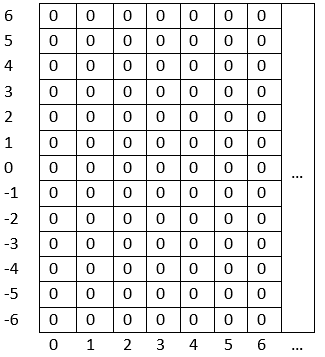
\includegraphics[width=6cm]{images/AccumulatorSpace.PNG}
		\label{tab:AccumulatorSpace}
	\end{minipage}
\end{adjustbox}\\

\noindent Pada tabel \ref{tab:AccumulatorSpace}, sumbu X menggambarkan \textit{theta} sedangkan sumbu Y menggambarkan \textit{rho}.

\noindent Diasumsikan baris 1 dan kolom 1 adalah x = 0 dan y = 0. Misalkan dilakukan pengecekan untuk baris 1 kolom 1. Ternyata baris 1 kolom 1 memiliki nilai 255 (objek berwarna putih) karena itu dihitung nilai \textit{rho} untuk sudut 0 hingga 180 derajat. Berikut adalah uraiannya:
\begin{enumerate}
\item Untuk sudut 0 derajat:\\
$\rho = x * \cos{\theta} + y * \sin{\theta}$\\
$\rho = 0 * \cos{0} + 0 * \sin{0}$\\
$\rho = 0 * 1 + 0 * 0$\\
$\rho = 0$\\
Tambahkan nilai \textit{voting} untuk \textit{rho} = 0 dengan \textit{theta} = 0 sebesar 1.
\item Untuk sudut 1 derajat:\\
$\rho = x * \cos{\theta} + y * \sin{\theta}$\\
$\rho = 0 * \cos{1} + 0 * \sin{1}$\\
$\rho = 0 * 0,99984 + 0 * 0,01745$\\
$\rho = 0$\\
Tambahkan nilai \textit{voting} untuk \textit{rho} = 0 dengan \textit{theta} = 1 sebesar 1.
\item Untuk sudut 2 derajat:\\
$\rho = x * \cos{\theta} + y * \sin{\theta}$\\
$\rho = 0 * \cos{2} + 0 * \sin{2}$\\
$\rho = 0 * 0,99939 + 0 * 0,03489$\\
$\rho = 0$\\
Tambahkan nilai \textit{voting} untuk \textit{rho} = 0 dengan \textit{theta} = 2 sebesar 1.
\item Untuk sudut 3 derajat:\\
$\rho = x * \cos{\theta} + y * \sin{\theta}$\\
$\rho = 0 * \cos{3} + 0 * \sin{3}$\\
$\rho = 0 * 0,99862 + 0 * 0,05233$\\
$\rho = 0$\\
Tambahkan nilai \textit{voting} untuk \textit{rho} = 0 dengan \textit{theta} = 3 sebesar 1.
\item Untuk sudut 4 derajat:\\
$\rho = x * \cos{\theta} + y * \sin{\theta}$\\
$\rho = 0 * \cos{4} + 0 * \sin{4}$\\
$\rho = 0 * 0,99756 + 0 * 0,06975$\\
$\rho = 0$\\
Tambahkan nilai \textit{voting} untuk \textit{rho} = 0 dengan \textit{theta} = 4 sebesar 1.
\item Untuk sudut 5 derajat:\\
$\rho = x * \cos{\theta} + y * \sin{\theta}$\\
$\rho = 0 * \cos{5} + 0 * \sin{5}$\\
$\rho = 0 * 0,99619 + 0 * 0,08715$\\
$\rho = 0$\\
Tambahkan nilai \textit{voting} untuk \textit{rho} = 0 dengan \textit{theta} = 5 sebesar 1.
\item Untuk sudut 6 derajat:\\
$\rho = x * \cos{\theta} + y * \sin{\theta}$\\
$\rho = 0 * \cos{6} + 0 * \sin{6}$\\
$\rho = 0 * 0,99452 + 0 * 0,10452$\\
$\rho = 0$\\
Tambahkan nilai \textit{voting} untuk \textit{rho} = 0 dengan \textit{theta} = 6 sebesar 1.
\end{enumerate}

\noindent Cara di atas diulang untuk 7 derajat hingga 180 derajat.

\noindent Setelah menyelesaikan perhitungan untuk titik koordinat (0,0) maka berikut adalah perubahan yang ditunjukan oleh matriks \textit{accumulator space}:

\begin{adjustbox}{width=1\textwidth}
	\noindent\begin{minipage}{\linewidth}
		\captionof{table}{Nilai \textit{voting} koordinat (0,0) disimpan di matriks \textit{Accumulator Space}\\}
		\centering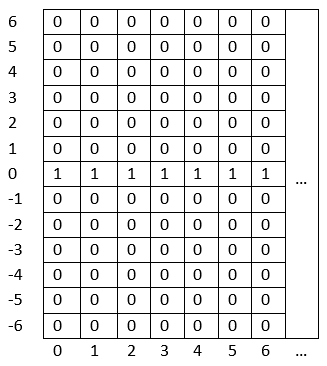
\includegraphics[width=6cm]{images/AccumulatorSpace1.PNG}
		\label{tab:AccumulatorSpaceAfterVoting}
	\end{minipage}
\end{adjustbox}\\

\noindent Proses di atas diulangi untuk semua piksel (nilai x dan y yang berbeda) dalam citra (hanya piksel yang bernilai 255 saja yang dihitung jaraknya). Jika sudah diterapkan untuk setiap kombinasi x dan y maka keluaran yang didapat adalah:

\begin{adjustbox}{width=1\textwidth}
	\noindent\begin{minipage}{\linewidth}
		\captionof{table}{Matriks \textit{Accumulator Space} dan nilai \textit{voting} yang disimpan\\}
		\centering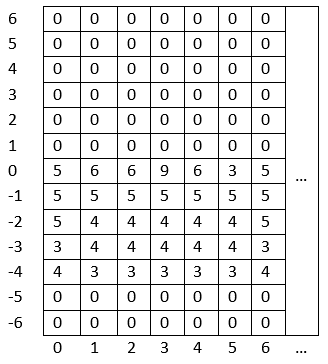
\includegraphics[width=6cm]{images/AccumulatorSpace2.PNG}
		\label{tab:AccumulatorSpaceAfterAllVoting}
	\end{minipage}
\end{adjustbox}\\

\noindent Setelah mendapat matriks \textit{accumulator space} selanjutnya adalah mencari nilai \textit{Hough Peaks}. Untuk menentukan nilai \textit{Hough Peaks} diperlukan untuk menentukan nilai \textit{threshold}, \textit{neighbourhood}, dan jumlah \textit{peaks}. Misalkan dalam kasus ini ditentukan nilai \textit{threshold} = 3, neighbourhood = 1, dan \textit{peaks} = 3, maka:
\begin{enumerate}
\item Dicari nilai yang memiliki nilai \textit{vote} di atas nilai \textit{threshold}, maka nilai pertama yang diperiksa adalah (diberi warna oranye):\\
\begin{adjustbox}{width=1\textwidth}
	\noindent\begin{minipage}{\linewidth}
		\captionof{table}{Koordinat (0,0) memiliki nilai di atas \textit{threshold}\\}
		\centering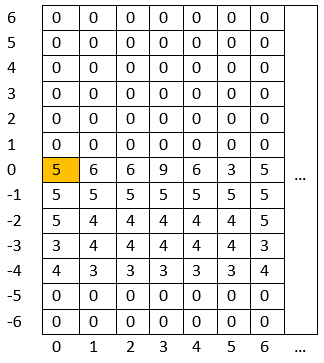
\includegraphics[width=6cm]{images/AccumulatorSpace3.PNG}
		\label{tab:AccumulatorSpaceFirstCheck}
	\end{minipage}
\end{adjustbox}\\
\item Memeriksa \textit{neighbour} apakah terdapat nilai vote yang memiliki nilai \textit{vote} lebih tinggi, jika ada tetangganya yang memiliki nilai \textit{vote} lebih tinggi maka nilai tersebut ditolak dan sebaliknya jika tidak maka nilai tersebut dipilih sebagai peak:\\
\\
\begin{adjustbox}{width=1\textwidth}
	\noindent\begin{minipage}{\linewidth}
		\captionof{table}{Memeriksa \textit{neighbour} dari koordinat (0,0)\\}
		\centering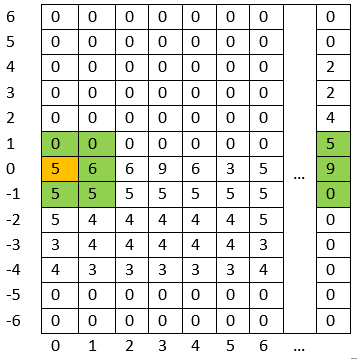
\includegraphics[width=6cm]{images/AccumulatorSpace4.PNG}
		\label{tab:AccumulatorSpaceNeighbourCheck}
	\end{minipage}
\end{adjustbox}\\
\\
Karena tetangga dari (0,0) terdapat nilai \textit{vote} yang lebih tinggi dari 5 (nilai 9 pada (0,180)) maka nilai \textit{vote} pada (0,0) tidak diterima sebagai \textit{peak}. Cara di atas diulang hingga mendapatkan seluruh \textit{peak} potensial yang ada. Misalkan didapatkan 5 \textit{peak} potensial sebagai berikut:
\begin{table}[H]
	\centering
	\captionof{table}{\textit{Peak} yang belum terurut\\}
	\begin{small}
		\begin{tabular}{|p{3cm}|p{1cm}|p{1cm}|p{1cm}|p{1cm}|p{1cm}|}
			\hline
			\textbf{Peak} & 1 & 2 & 3 & 4 & 5\\
			\hline
			\textbf{Jumlah Voting} & 6 & 9 & 5 & 4 & 4\\
			\hline
			\textbf{\textit{Theta}} & 1 & 3 & 6 & 3 & 10 \\
			\hline
		\end{tabular}
	\end{small}
	\label{tab:PeakUnsorted}
\end{table}
Setelah mendapatkan sejumlah nilai \textit{peak} potensial kemudian \textit{peak} potensial tersebut diurutkan dari nilai terbesar hingga terkecil (\textit{descending}) berdasarkan nilai \textit{voting}. Maka nilai dari pengurutan \textit{peaks} potensial tersebut adalah:
\begin{table}[H]
	\centering
	\captionof{table}{\textit{Peak} terurut secara \textit{descending} berdasarkan jumlah \textit{voting}\\}
	\begin{small}
		\begin{tabular}{|p{3cm}|p{1cm}|p{1cm}|p{1cm}|p{1cm}|p{1cm}|}
			\hline
			\textbf{Peak} & 1 & 2 & 3 & 4 & 5\\
			\hline
			\textbf{Jumlah Voting} & 9 & 6 & 5 & 4 & 4\\
			\hline
			\textbf{\textit{Theta}} & 3 & 1 & 6 & 3 & 10 \\
			\hline
		\end{tabular}
	\end{small}
	\label{tab:PeakSorted}
\end{table}
\item Karena jumlah \textit{peaks} yang ditentukan adalah 3 maka ambil 3 \textit{peaks} dengan nilai \textit{voting} tiga tertinggi:
\begin{table}[H]
	\centering
	\captionof{table}{Tiga \textit{peaks} yang terpilih\\}
	\begin{small}
		\begin{tabular}{|p{3cm}|p{1cm}|p{1cm}|p{1cm}|}
			\hline
			\textbf{Peak} & 1 & 2 & 3\\
			\hline
			\textbf{Jumlah Voting} & 9 & 6 & 5\\
			\hline
			\textbf{\textit{Theta}} & 3 & 1 & 6\\
			\hline
		\end{tabular}
	\end{small}
	\label{tab:ChosenPeak}
\end{table}
\item Setelah mendapatkan sejumlah \textit{peaks} yang diinginkan berikutnya adalah menghitung intensitas kemunculan dari setiap nilai \textit{theta} (rentang niali \textit{theta} yang digunakan adalah 0-180 derajat). Misalkan hasil perhitungan intensitas kemunculan tersebut adalah:
\begin{table}[H]
	\centering
	\captionof{table}{Intensitas kemunculan dari setiap nilai \textit{theta}\\}
	\begin{small}
		\begin{tabular}{|p{2cm}|p{1cm}|p{1cm}|p{1cm}|p{1cm}|p{1cm}|p{1cm}|p{1cm}|p{1cm}|p{1cm}|}
			\hline
			\textbf{Theta} & 0 & 1 & 2 & 3 & 4 & 5 & 6 & \dots & 180\\
			\hline
			\textbf{Intensitas Kemunculan} & 0 & 1 & 0 & 1 & 0 & 0 & 1 & \dots &0\\
			\hline
		\end{tabular}
	\end{small}
	\label{tab:ChosenPeak}
\end{table}
\noindent Keluaran dari metode \textit{Hough Transform} ini adalah kumpulan nilai \textit{rho} dan \textit{theta} yang nantinya akan digunakan untuk mencari seluruh kandidat garis. Dari kandidat garis tersebut akan didapatkan garis vertikal dan garis horizontal, dengan menggunakan perhitungan \textit{Euclidean Distance} seluruh garis vertikal akan dikelompokkan dan diperiksa manakah dari kelompok garis yang memiliki koordinat titik awal dan titik akhir yang hampir sama. Kemudian titik awal dan titik akhir dari kedua garis tersebut akan digabungkan menjadi bentuk persegi panjang dan area tersebut yang akan disebut dengan area plat kendaraan.\\
\begin{adjustbox}{width=1\textwidth}
	\noindent\begin{minipage}{\linewidth}
		\centering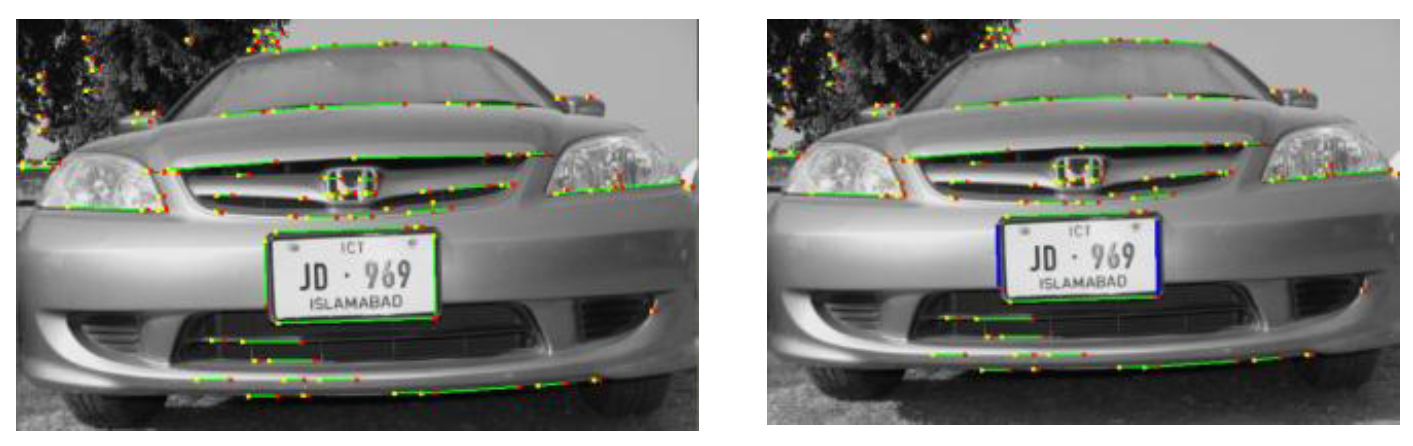
\includegraphics[width=11cm]{images/SeleksiKandidatGaris.PNG}
		\captionof{figure}{Seleksi Kandidat Garis\\}
		\label{fig:SeleksiKandidatGaris}
	\end{minipage}
\end{adjustbox}\\
\\
\begin{adjustbox}{width=1\textwidth}
	\noindent\begin{minipage}{\linewidth}
		\centering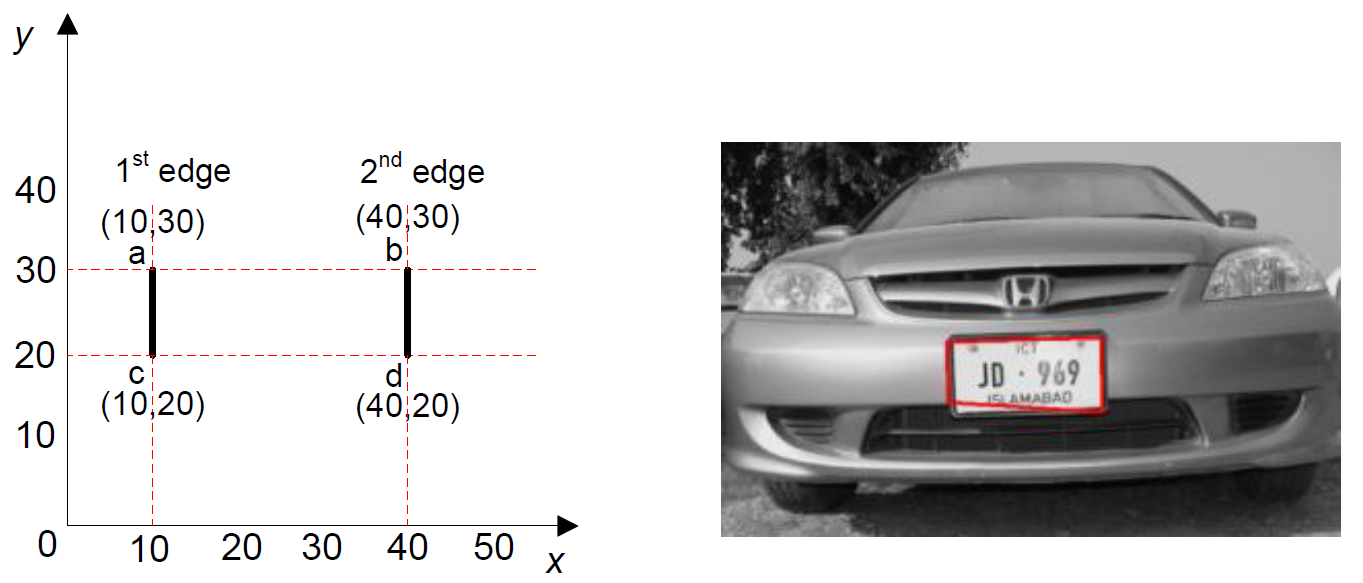
\includegraphics[width=11cm]{images/AreaPlatKendaraan.PNG}
		\captionof{figure}{Penentuan Area Plat Kendaraan\\}
		\label{fig:Penentuan Area Plat Kendaraan}
	\end{minipage}
\end{adjustbox}\\
\\
\end{enumerate}

\subsection{Tahapan Segmentasi Karakter}
\noindent Pada tahapan segmentasi karakter, akan dilakukan dua tahapan, yaitu segmentasi vertikal untuk mendapatkan batas atas dan batas bawah daerah karakter, dan segmentasi horizontal untuk mendapatkan batas kiri dan batas kanan untuk setiap karakter.

\noindent Pada penelitian ini, tahapan segmentasi karakter akan menggunakan \textit{library} dari Java OCR.\\

\subsection{\textit{Histogram of Oriented Gradient}}
\noindent Pada proses \textit{Histogram of Oriented Gradients}, masukan untuk proses ini berupa citra yang berasal dari hasil \textit{preprocessing}. Keluaran dari proses ini adalah matriks fitur vektor dari hasil perhitungan \textit{Histogram of Oriented Gradients}. Berikut merupakan langkah-langkah untuk menghitung matriks fitur vektor. Pada gambar dapat dilihat hasil dari proses \textit{resize} dan \textit{crop} citra \textit{grayscale} berukuran 8 $\times$ 4 piksel.

\begin{table}[H]
	\centering
	\begin{small}
		\begin{tabular}{|p{2cm}|p{2cm}|p{2cm}|p{2cm}|}
			\hline
			89 & 92 & 88 & 92 \\
			\hline
			90 & 88 & 90 & 86 \\
			\hline
			91 & 90 & 90 & 94 \\
			\hline
			91 & 122 & 91 & 122 \\
			\hline
			89 & 90 & 89 & 91 \\
			\hline
			90 & 85 & 90 & 86 \\
			\hline
			91 & 90 & 92 & 93 \\
			\hline
			91 & 122 & 91 & 120 \\
			\hline
		\end{tabular}
	\end{small}
	\captionof{figure}{Matriks citra hasil \textit{preprocessing}\\}
	\label{fig:MatriksCitraHasilPreprocessing}
\end{table}

\begin{enumerate}
\item Proses pertama adalah untuk menghitung nilai gradien dari posisi vertikal dan horizontal untuk setiap piksel menggunakan persamaan \ref{eq:PersamaanGradienX} dan \ref{eq:PersamaanGradienY}. Contoh perhitungannya untuk piksel koordinat (2,5) dan hasil dari tahap ini dapat dilihat pada gambar \ref{fig:MatriksCitraHasilGradienX} dan \ref{fig:MatriksCitraHasilGradienY} di bawah:
\begin{equation*}
	G_{x}(2,5) = 89 - 89 = 0
\end{equation*}
\begin{equation*}
	G_{y}(2,5) = 85 - 122 = -37
\end{equation*}
\begin{table}[H]
	\centering
	\begin{small}
		\begin{tabular}{|p{2cm}|p{2cm}|p{2cm}|p{2cm}|}
			\hline
			0 & -1 & 0 & 0 \\
			\hline
			0 & 0 & -2 & 0 \\
			\hline
			0 & -1 & 4 & 0 \\
			\hline
			0 & 0 & 0 & 0 \\
			\hline
			0 & 0 & 1 & 0 \\
			\hline
			0 & 0 & 1 & 0 \\
			\hline
			0 & 1 & 3 & 0 \\
			\hline
			0 & 0 & -2 & 0 \\
			\hline
		\end{tabular}
	\end{small}
	\captionof{figure}{Matriks hasil Perhitungan Gradien sumbu X\\}
	\label{fig:MatriksCitraHasilGradienX}
\end{table}
\begin{table}[H]
	\centering
	\begin{small}
		\begin{tabular}{|p{2cm}|p{2cm}|p{2cm}|p{2cm}|}
			\hline
			0 & 0 & 0 & 0 \\
			\hline
			2 & -2 & 2 & 2 \\
			\hline
			1 & 34 & 1 & 36 \\
			\hline
			-2 & 0 & -1 & -3 \\
			\hline
			-1 & -37 & -1 & -36 \\
			\hline
			2 & 0 & 3 & 2 \\
			\hline
			1 & 37 & 1 & 34 \\
			\hline
			0 & 0 & 0 & 0 \\
			\hline
		\end{tabular}
	\end{small}
	\captionof{figure}{Matriks hasil Perhitungan Gradien sumbu Y\\}
	\label{fig:MatriksCitraHasilGradienY}
\end{table}
\item Untuk setiap piksel, hitung \textit{magnitude} gradien dan arah gradien menggunakan persamaaan \ref{eq:PersamaanMagnitude} dan \ref{eq:PersamaanArah}. Contoh perhitungannya untuk piksel koordinat (2,5) dan hasil dari tahap ini dapat dilihat pada gambar di bawah:
\begin{equation*}
M(2,5) = \sqrt{0^2 + (-37)^2} = 37
\end{equation*}
\begin{equation*}
\theta(2,5) = arctan\frac{-37}{0} = 90
\end{equation*}
\begin{table}[H]
	\centering
	\begin{small}
		\begin{tabular}{|p{2cm}|p{2cm}|p{2cm}|p{2cm}|}
			\hline
			0 & 1 & 0 & 0 \\
			\hline
			2 & 2 & 2 & 2 \\
			\hline
			1 & 34 & 4 & 36 \\
			\hline
			2 & 0 & 1 & 3 \\
			\hline
			1 & 37 & 1 & 36 \\
			\hline
			2 & 0 & 3 & 2 \\
			\hline
			1 & 37 & 3 & 34 \\
			\hline
			0 & 0 & 2 & 0 \\
			\hline
		\end{tabular}
	\end{small}
	\captionof{figure}{Matriks hasil Perhitungan \textit{Magnitude}\\}
	\label{fig:MatriksHasilMagnitude}
\end{table}
\begin{table}[H]
	\centering
	\begin{small}
		\begin{tabular}{|p{2cm}|p{2cm}|p{2cm}|p{2cm}|}
			\hline
			90 & 0 & 90 & 90 \\
			\hline
			90 & 90 & 45 & 90 \\
			\hline
			90 & 89 & 14 & 90 \\
			\hline
			90 & 90 & 90 & 90 \\
			\hline
			90 & 90 & 45 & 90 \\
			\hline
			90 & 90 & 71 & 90 \\
			\hline
			90 & 88 & 18 & 90 \\
			\hline
			90 & 90 & 0 & 90 \\
			\hline
		\end{tabular}
	\end{small}
	\captionof{figure}{Matriks hasil Perhitungan Arah\\}
	\label{fig:MatriksHasilPerhitunganArah}
\end{table}
\item Kemudian, tentukan ukuran sel, ukuran blok dan jumlah \textit{oriented histogram bins}. Pada penelitian Dalas dan Triggs untuk mendeteksi pejalan kaki sebelumnya, didapat bahwa ukuran sel sebesar 8 $\times$ 8 piksel, ukuran blok sebesar 2 $\times$ 2 ukuran sel dan jumlah bin sebanyak 9 sudah dapat menghasilkan akurasi yang dapat mendeteksi pejalan kaki dengan cukup baik dibandingkan dengan ukuran-ukuran lainnya. Untuk contoh perhitungan analisis kali ini jumlah \textit{oriented histogram bins} yang dipakai sebanyak 4 buah, sehingga didapat nilai sudut setiap \textit{histogram bin} yaitu 180 / 4 = 45. Untuk ukuran sel dipilih sebesar 2 $\times$ 2 piksel dan ukuran blok sebesar 2 $\times$ 2 sel.
\item Kemudian untuk setiap sel, tentukan perhitungan \textit{Histogram of Oriented Gradient} dengan melakukan \textit{voting} dari arah gradien dan \textit{magnitude} gradien, dimana arah gradien akan menjadi sudut \textit{bin}, dan \textit{magnitude} gradien akan menjadi bobot nilai. Berikut merupakan contoh proses \textit{voting} untuk piksel dengan koordinat (2,5).
\begin{equation*}
M(2,5) = 37
\end{equation*}
\begin{equation*}
\theta(2,5) = 90
\end{equation*}
Sehingga untuk \textit{bin} dengan sudut 90 akan mendapat nilai bobot sebesar 37 yang didapatkan dari nilai gradien \textit{magnitude}-nya.
Lakukan proses tersebut untuk setiap sel sehingga masing-masing sel akan mempunyai \textit{Histogram of Oriented Gradient}. Berikut contoh hasil perhitungan metode \textit{Histogram of Oriented Gradient} pada sel yang terdapat koordinat piksel (2,5) dapat dilihat pada gambar \ref{fig:HasilHOG}.\\
\begin{adjustbox}{width=1\textwidth}
	\noindent\begin{minipage}{\linewidth}
		\framebox[\textwidth]{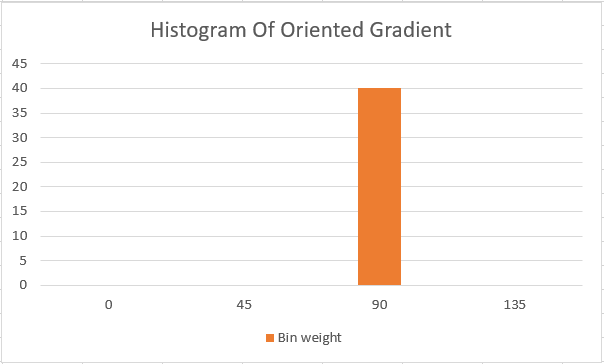
\includegraphics[width=12cm]{images/HistogramOfOrientedGradient.PNG}}
		\captionof{figure}{Contoh hasil \textit{Histogram of Oriented Gradient} untuk sel yang memiliki piksel dengan koordinat (2,5)}
		\label{fig:HasilHOG}
	\end{minipage}
\end{adjustbox}
\item Kemudian untuk setiap blok, akan dilakukan normalisasi dengan menggabungkan hasil histogram dari setiap sel dalam bloknya. Adapun proses normalisasi dapat menggunakan 4 algoritme yaitu, \textit{L1-Norm}, \textit{L1-Sqrt}, \textit{L2-Norm}, dan \textit{L2-Hys}. Pada penelitian ini, penulis menggunakan algoritme normalisasi \textit{L2-Norm} karena berdasarkan penelitian sebelumnya, hasil yang didapat lebih baik dari algoritme lainnya. Persamaan algoritme untuk proses normalisasi menggunakan \textit{L2-Norm} didapat dengan menggunakan persamaan \ref{eq:L2-Norm}. Di bawah adalah contoh perhitungan normalisasi untuk blok pertama:
\begin{table}[H]
	\centering
	\begin{small}
		\begin{tabular}{|p{1cm}|p{1cm}|p{1cm}|p{1cm}|p{1cm}|p{1cm}|p{1cm}|p{1cm}|}
			\hline
			1 & 0 & 4 & 0 & 0 & 2 & 2 & 0 \\
			\hline
			0 & 0.76 & 36.24 & 0 & 2.76 & 1.24 & 40 & 0 \\
			\hline
			0 & 0 & 40 & 0 & 0 & 2.27 & 39.73 & 0 \\
			\hline
			0 & 1.65 & 36.35 & 0 & 3.8 & 1.2 & 34 & 0 \\
			\hline
		\end{tabular}
	\end{small}
	\captionof{figure}{Matriks hasil Perhitungan Histogram untuk seluruh sel\\}
	\label{fig:MatriksHasilPerhitunganHistogram}
\end{table}
Berdasarkan matriks pada gambar \ref{fig:MatriksHasilPerhitunganHistogram}. Elemen matriks yang akan kita gunakan dalam perhitungan normalisasi ini adalah seluruh elemen baris pertama dan baris kedua.
\begin{equation*}
L2_{Norm} = \sqrt{1^2 + 0^2 + \ldots + 2^2 + 0^2 + 0^2 + 0.76^2 + \ldots + 40^2 + 0^2} = 54.29
\end{equation*}
Kemudian untuk setiap nilai dari histogram dari sel dalam blok tersebut akan dibagi dengan nilai hasil normalisasinya. Di bawah adalah contoh hasil normalisasi histogram dari sel pertama (matriks hasil perhitungan histogram baris pertama kolom 1-4):
\begin{gather*}
\begin{bmatrix}
0.018418 & 0 & 0.07367 & 0 \\
\end{bmatrix}
\end{gather*}
Lakukan proses normalisasi untuk setiap blok dengan menggeser secara horizontal sejauh 1 kali ukuran sel dan secara vertikal sejauh 1 kali ukuran sel sampai blok tersebut sudah berada di bawah kanan dari citra. Kemudian hasil dari proses normalisasi akan disusun menjadi matriks besar dengan jumlah kolom sebesar  \textit{jumlah bin} $\times$ \textit{lebar blok dalam satuan sel} $\times$ \textit{jumlah pergeseran horizontal} dan jumlah baris sebesar \textit{jumlah pergeseran vertikal} $\times$ \textit{tinggi blok dalam satuan sel} , dengan perhitungan tersebut, dalam analisa saat ini didapatkan ukuran matriks sebesar 6 $\times$ 8. Dalam analisa ini, hasil keluaran dari metode \textit{Histogram of Oriented Gradient} ada sebanyak 48 fitur. Di bawah adalah hasil fitur vektor untuk metode \textit{Histogram of Oriented Gradient} setelah melewati proses normalisasi.\\
\begin{table}[H]
	\centering
	\begin{small}
		\begin{tabular}{|p{1cm}|p{1cm}|p{1cm}|p{1cm}|p{1cm}|p{1cm}|p{1cm}|p{1cm}|}
			\hline
			0.0184 & 0 & 0.0736 & 0 & 0 & 0.0368 & 0.0368 & 0\\
			\hline
			0 & 0.0139 & 0.6674 & 0 & 0.0508 & 0.0228 & 0.7367 & 0\\
			\hline
			0 & 0.0097 & 0.4637 & 0 & 0.0353 & 0.0158 & 0.5118 & 0\\
			\hline
			0 & 0 & 0.5118 & 0 & 0 & 0.0290 & 0.5084 & 0 \\
			\hline
			0 & 0 & 0.5307 & 0 & 0 & 0.0301 & 0.5271 & 0 \\
			\hline
			0 & 0.0218 & 0.4823 & 0 & 0.0504 & 0.0159 & 0.4511 & 0 \\
			\hline
		\end{tabular}
	\end{small}
	\captionof{figure}{Matriks hasil Normalisasi\\}
	\label{fig:MatriksHasilNormalisasi}
\end{table}
Setelah mendapatkan matriks \textit{HOG descriptor} di atas. Langkah berikutnya adalah menjadikan matriks tersebut sebagai vektor. Hal ini dilakukan dengan mengambil setiap baris dari matriks dan memasukkannya ke dalam matriks vektor berukuran 1 $\times$ jumlah fitur. Vektor inilah yang akan dijadikan sebagai masukan bagi metode \textit{Machine Learning} yang akan digunakan dalam penelitian ini.\\
\end{enumerate}

\subsection{\textit{Support Vector Machine}}
\noindent \textit{HOG descriptor} yang dihasilkan dari perhitungan metode \textit{Histogram of Oriented Gradient} akan digunakan sebagai masukan \textit{Support Vector Machine}. \textit{Support Vector Machine} yang akan digunakan dalam penelitian menggunakan \textit{library} dari Weka SVM. \textit{Support Vector Machine} termasuk dalam algoritme \textit{supervised learning}. Konsep dasar dari metode ini adalah untuk menemukan sebuah \textit{separating hyperplane} (bidang) yang dapat memisahkan dua kelas sebagai keputusan klasifikasi. Dalam penelitian ini karakter yang akan dikenali adalah huruf A sampai dengan Z dan angka dari 0 sampai dengan 9 sehingga akan terdapat 36 kelas untuk proses klasifikasi.
%\noindent Tabel \ref{tbl:filteredDataset} merupakan rincian jumlah citra pada masing-masing \textit{dataset} setelah dilakukan pemilihan.
%\begin{table}[H]
%	\centering
%	\begin{small}
%		\captionof{table}{Rincian \textit{Dataset} yang telah dipilih\label{tbl:filteredDataset}}
%		\begin{tabular}{|p{4cm}|p{1cm}|p{3cm}|p{3cm}|}
%			\hline
%			\textbf{Nama \textit{Dataset}} &\textbf{Folder} & \textbf{Jumlah Citra} & \textbf{Jumlah Posisi Manusia}\\
%			\hline
%			\textit{Clothing Store} 			& - & 770 & 1631 \\
%			\hline
%			\multirow{3}{*}\textit{Outdoor}	& 31 & 46 & 218 \\\cline{2-4}
%			& 54 & 84 & 371 \\\cline{2-4}
%			& 56 & 113 & 496 \\\hline
%		\end{tabular}
%	\end{small}
%\end{table}



\newpage